\section{Cyclic Redundancy Check (CRC)}

  CRC-Codes sind gut für eine Kanalcodierung um sporadische Fehler wie Rauschen zu detektieren. Sie
  eignen sich aber nicht um systematische Datenmanipulationen festzustellen.

\subsection{Blockcodes \buch{p.5}}
  \begin{itemize}
    \item Blockcodes erzeugen aus k Datenbits (Eingangssymbole) n Codebits (Ausgangssymbole).
          Dies ergibt ein (n,k)-Code.
    \item Jeder Block aus den k Datenbits wird eigenständig codiert, dadurch wird der Block erkennungs-
          und korrekturfähig.
    \item Ein Blockcode ist linear, wenn die Modulo-2 Addition (EXOR Verknüpfung) zweier beliebiger gültiger
          Codeworte wieder ein neues Codewort ergibt.
    \item Alle $2^k$ möglichen Blocks der Länge k werden eindeutig auf $2^k$ Codeworte der Länge n abgebildet.
    \item \textbf{Zyklische Codes} sind eine Untergruppe der linearen Blockcodes. Sie haben einen einfachen
          Hardwareaufbau (z.B Hamming-Codes).
  \end{itemize}

\subsection{Prüfsequenz bestimmen}
  \begin{multicols}{2}
    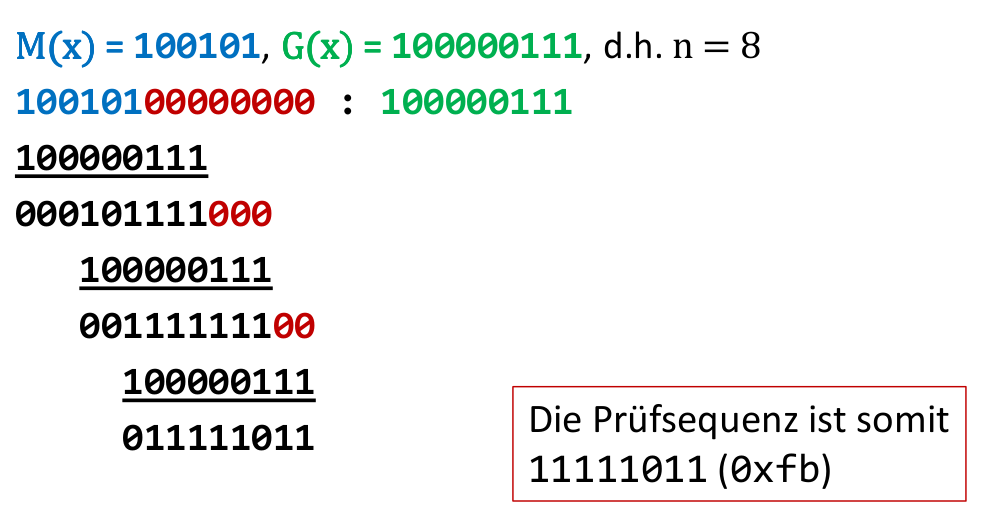
\includegraphics[width=10cm]{images/CRC/CRCRechenBsp}
    
  \columnbreak

    Codewort:\\
    $\underline{c} = (c_0, c_1, \ldots, c_{n-1})$ \\
    
    Zugehöriges Polynom:\\
    $c(x) = c_0 + c_1x + \ldots + c_{n-1}x^{n-1}$\\
    
    Beispiel:\\
    $\underline{c} = (1,0,0,1,1,0) \Rightarrow c(x) = 1 + x^3+x^4$    
  \end{multicols}
  
\subsection{typische Generator Polynome}
  \begin{tabular}{|p{3.5cm} l p{10cm}|}
  \hline
    \textbf{Bezeichnung} &
    \textbf{Polynom} & 
    \textbf{Verwendung}\\
  \hline
    CRC-8-CCITT & 
    0x107 & 
    ATM, ISDN \\
  \hline
    CRC-16-CCITT \newline (aka CRC-CCITT) &
    0x11021 &
    Bluetooth, SD-Card \\
  \hline
    CRC-16 \newline (aka CRC-16-ANSI, CRC-16-IBM) &
    0x18005 &
    Modbus, USB \\
  \hline
    CRC-32 \newline (aka CRC-32-IEEE) &
    0x104C11DB7 &
    Ethernet, ZIP, Serial ATA, HDLC, MPEG-2, PNG, u.a\\
  \hline
  \end{tabular}\\
  
  Da das MSB des Polynoms immer 1 ist, wird dies häufig bei der Beschreibung weggelassen, z.B 0x8005 statt
  0x18005 beim CRC-16. \newline
  Das LSB wird teilweise auch weggelassen, da dies ebenfalls immer 1 ist.
  
\subsection{Implementation}
\subsubsection{Bit by Bit}
\begin{lstlisting}[style=Cpp]
Crc crcSlow(const uint8_t message[], unsigned int nBytes)
{
  Crc remainder = 0;
  Crc crcPoly = 0x07;
  unsigned int byte;
  unsigned int bit;
  for (byte = 0; byte < nBytes; ++byte){
    remainder ^= message[byte];
    for (bit = 8; bit > 0; --bit){
      if (remainder & crcTopBit)
        remainder = (remainder << 1) ^ crcPoly;
      else
        remainder = (remainder << 1);
    }
  }
  return remainder;
}
\end{lstlisting}

\subsubsection{Tabelle}
\begin{lstlisting}[style=Cpp]
Crc crcFast(const uint8_t message[], unsigned int nBytes)
{
  Crc remainder = 0;
  uint8_t data;
  unsigned int byte;
  for (byte = 0; byte < nBytes; ++byte){
    data = message[byte] ^ remainder;
    remainder = crcTable[data];
  }
  return remainder;
}
\end{lstlisting}



